% draft会跳过文档中的所有图片。正式导出时需要删掉draft参数。
\documentclass[12pt, a4paper, oneside]{ctexart}

\usepackage{amsmath}
\usepackage{amssymb}
\usepackage{bm}
\usepackage{graphicx}
\usepackage{mathrsfs}
\usepackage{geometry}
\usepackage{framed}
\usepackage{color}
\usepackage[dvipsnames]{xcolor}
\usepackage{caption}
\usepackage{listings}
\usepackage{fancyhdr}
\usepackage{booktabs}
\usepackage{makecell}
\usepackage{indentfirst}
\usepackage{authblk}
\usepackage{multicol}
% \usepackage{draftwatermark}       % 需要应用水印时取消注释
\usepackage{enumitem}
\usepackage[hidelinks]{hyperref}
\usepackage{tikz}
\usepackage{ulem}
\usetikzlibrary{positioning, shapes.geometric}

% 分栏线宽
\columnseprule=0.4pt

% 定制第二级无序列表的点样式
\setlist[itemize,2]{label=$\diamond$}

% 页边距
\geometry{a4paper, scale=0.8}

\pagestyle{fancy}

\fancyhf{}      % 清空页眉页脚设置
\fancyhead[L] {
    % 工大计算机系logo
    
\includegraphics[height=7mm]{./images/logo1.jpg}
}
\fancyhead[C]{《操作系统》复习}
\fancyhead[R]{\leftmark}    % 右侧页眉:当前章标题

% 页脚居中放置页码
\fancyfoot[C]{\thepage}

% 设置章节标题自动编号的格式
\ctexset{
  section/number=\chinese{section},
%   subsection/name={,},
%   subsection/number=\chinese{subsection}
}

% 行距。ctexart默认值为1.3
\linespread{1.2}

\lstset{
  language=c,
  basicstyle=\ttfamily,
  frame=single,
  % keywordstyle=\bfseries\color{NavyBlue}  % 彩色看起来怪怪的,所以注释掉了
  numbers=left, % 显示行号在左边
  numbersep=2em, % 设置行号的具体位置
  numberstyle=\footnotesize, % 缩小行号
  frame=single, % 边框
  framesep=1em % 设置代码与边框的距离
}

% \SetWatermarkText{Eslzzyl整理}            % 设置水印内容
% \SetWatermarkLightness{0.9}             % 设置水印透明度 0-1
% \SetWatermarkScale{0.8}                   % 设置水印大小 0-1

\renewcommand{\headrulewidth}{1pt}  %页眉线宽,设为0可以去页眉线
\renewcommand{\footrulewidth}{1pt}  %脚注线的宽度

\definecolor{shadecolor}{RGB}{241, 241, 255}

\title{
    
\includegraphics[width=0.3\textwidth]{images/hfut-badge.pdf}
    
    \vspace{20pt}
    《操作系统》总复习
}
\author{Eslzzyl}
\date{\today}

\newcounter{problemname}
\newenvironment{problem}{\begin{shaded}\stepcounter{problemname}\par\noindent\textbf{例题\arabic{problemname}. }}{\end{shaded}\par}
\newenvironment{solution}{\begin{shaded}\par\noindent\textbf{解答:}}{\end{shaded}\par}
% \newenvironment{solution}{\par\noindent\textbf{答案. }}{\par}
% \newenvironment{note}{\par\noindent\textbf{例题\arabic{problemname}的注记. }}{\\\par}
\newenvironment{note}{\par\noindent\textbf{注记. }}{\par}

\begin{document}

\maketitle
\newpage
\tableofcontents
\vspace{20pt}
% 如果在目录处有备注,可以写在这里。

\newpage

\section{计算机系统概述}

本章主要是选择题。

\subsection{操作系统的基本概念}

\subsubsection{操作系统的概念}

计算机系统\textbf{自上而下}可分为4层:
\begin{enumerate}
  \item 用户
  \item 应用程序
  \item 操作系统
  \item 硬件
\end{enumerate}

操作系统的\textbf{定义}:操作系统是一组管理和控制计算机软件和硬件资源,合理组织计算机系统工作流程,以及方便用户使用的\textbf{程序的集合}。

OS是计算机系统中最基本的系统软件。

\subsubsection{操作系统的特征}

四大基本特征:
\begin{itemize}
  \item {\bf 并发(Concurrence)}
  \begin{itemize}
    \item 并发:多个事件在同一时间间隔内发生。
    \item 并行:多个事件在同一时刻发生。
  \end{itemize}
  操作系统的并发性是通过分时得以实现的。
  \item {\bf 共享(Sharing)}
  \begin{itemize}
    \item 互斥共享方式
    \item 同时访问方式
  \end{itemize}
  \item {\bf 虚拟(Virtual)}
  
  虚拟技术有两种实现方式:
  \begin{itemize}
    \item 时分复用技术,如处理器的分时共享;
    \item 空分复用技术,如虚拟存储器。
  \end{itemize}
  \item {\bf 异步(Asynchronism)}
  
  多道程序环境下,程序的执行是走走停停的,即以不可知的速度向前推进,这就是进程的异步性。OS必须保证在相同的运行环境下,进程多次运行的结果是一致的。
\end{itemize}

并发和共享是OS的最基本特性。

\subsubsection{操作系统的目标和功能}

\begin{enumerate}
  \item 系统资源的\textbf{管理}者
  \begin{itemize}
    \item 处理机管理,也就是对进程的管理,包括
    \begin{itemize}
      \item 进程控制
      \item 进程同步
      \item 进程通信
      \item 死锁处理
      \item 处理机调度
    \end{itemize}
    \item 存储器管理
    \begin{itemize}
      \item 内存分配与回收
      \item 地址映射
      \item 内存保护和共享
      \item 内存扩充
    \end{itemize}
    \item 文件管理
    \begin{itemize}
      \item 文件存储空间的管理
      \item 目录管理
      \item 文件读写管理和保护
    \end{itemize}
    \item 设备管理
    \begin{itemize}
      \item 缓冲管理
      \item 设备分配
      \item 设备处理
      \item 虚拟设备
    \end{itemize}
  \end{itemize}
  \item 作为用户和硬件系统之间的\textbf{接口}
  \begin{itemize}
    \item 命令接口
    \begin{itemize}
      \item 联机方式:交互式
      \begin{itemize}
        \item 字符式
        \item 图形用户接口GUI
      \end{itemize}
      \item 脱机方式:批处理式
    \end{itemize}
    \item 程序接口:由一组系统调用组成
  \end{itemize}
  \item 实现对计算机资源的\textbf{扩充}
\end{enumerate}

\subsection{操作系统发展历程}

推动OS发展的主要动力:
\begin{itemize}
  \item 不断提高计算机资源利用率
  \item 方便用户
  \item 器件的不断更新换代
  \item 计算机体系结构的发展
  \item 不断提出新的应用需求
\end{itemize}

\subsubsection{无操作系统时代}

对计算机的所有操作采用人工操作方式完成。人工操作方式的缺点:
\begin{itemize}
  \item 用户独占全机
  \item CPU等待人工操作
\end{itemize}

由于以上两点,昂贵的机器资源在大部分时间内处于空闲状态,非常浪费。

优点:交互性好,即用户可以得到机器的立即响应。

\subsubsection{单道批处理系统}

\textbf{批处理系统}:在计算机上加载一个专门监控软件,在其控制下,计算机
能够自动地、成批地处理一个或多个用户的一批作业。

批处理系统的特点:
\begin{itemize}
  \item 系统吞吐量大
  \item 资源利用率高
  \item 平均周转时间短
  \item 无交互能力(缺点)
\end{itemize}

\textbf{单道批处理系统}:先把一批作业输入到磁带上,在监控程序的控制下使这批作业一个接一个地处理。
内存中始终只保持一道作业。

代表系统:IBM的FMS(Fortran Monitoring System),1960s

一定程度上改善了资源浪费,但失去了交互性。单个程序独占系统,程序I/O时CPU空等。

单道批处理系统的特点:自动性、顺序性、单道性

\subsubsection{多道批处理系统}

出现的动力是希望提高资源利用率和系统吞吐量。

代表系统(也是第一个):IBM的OS/360,1960s

由作业调度程序按照一定的算法,从后备队列中选择若干个作业调入内存,使它们共享CPU资源。

相比单道批处理系统,多道批处理系统的资源利用率更高,但仍然没有交互性。

特点:多道性、无序性、调度性、宏观上并行、微观上串行

\subsubsection{分时系统}

出现的动力是改善交互性。

分时系统:在一台主机上连接若干个终端,允许多个用户通过终端以交互方式共享主机资源。

代表系统:CTSS(1962)、Multics(1964)

特点:
\begin{itemize}
  \item 多路性:众多联机用户可以同时使用同一台计算机
  \item 独立性:各终端用户感觉到自己独占了计算机
  \item 及时性:用户的请求能在很短时间内得到响应
  \item 交互性:用户与计算机之间可进行“会话”
\end{itemize}

\subsubsection{实时系统}

实时计算:系统的正确性不仅由计算的逻辑结果来确定,而且还取决于产生结果的时间。

常见的实时系统:
\begin{itemize}
  \item 工业控制系统、武器控制系统
  \item 信息查询系统
  \item 多媒体系统
  \item 嵌入式系统
\end{itemize}

代表系统:WinCE,嵌入式Linux,ucOSII,VxWorks等

特点:实时性、高安全性、高可靠性(效率放第二位)、整体性强、会话能力要求不高

\subsubsection{网络操作系统和分布式计算机系统}

网络操作系统:将网络中的多台计算机连接起来。

分布式计算机系统:用于管理分布式计算机系统的操作系统。

\subsection{操作系统运行环境}

\subsubsection{处理器运行模式}

\begin{itemize}
  \item {\kaishu 特权指令},指不允许用户直接使用的指令。
  \item {\kaishu 非特权指令},指允许用户直接使用的指令。
\end{itemize}

CPU的运行模式:
\begin{itemize}
  \item {\kaishu 用户态}(目态)
  \item {\kaishu 内核态}(核心态、管态)
\end{itemize}

CPU在内核态可以执行特权指令,在用户态则只能执行非特权指令。应用程序运行在用户态,操作系统内核运行在内核态。

大多数操作系统内核包括:
\begin{itemize}
  \item 时钟管理
  \item 中断机制
  \item 原语
  \item 系统控制的数据结构及处理
\end{itemize}

\subsubsection{中断和异常的概念}

可直接参考《组成原理》相关内容。

\subsubsection{系统调用}

在用户程序中,凡与资源有关的操作,都必须使用系统调用。系统调用由OS内核完成,运行在核心态。

程序的运行由用户态转到核心态,需要用到访管指令,是用户态指令。

\subsection{操作系统结构}

\subsubsection{分层式结构OS}

原则:将功能模块分层,层内模块可以互相调用,层间模块只允许高层调用它下面紧邻着的那层,不允许反过来。

将最靠近硬件的低层OS部分称为操作系统内核,内核通常常驻主存。

优点:
\begin{itemize}
    \item 容易保证系统的正确性,容易调试和验证。
    \item 容易扩充、维护和移植。
\end{itemize}

缺点:
\begin{itemize}
  \item 效率低下。
  \item 合理定义各层比较困难。
\end{itemize}

\subsubsection{模块化结构OS}

优点:
\begin{itemize}
    \item 提高OS设计的正确性、可理解性和可维护性
    \item 增强OS的可移植性, 加速OS的开发过程
\end{itemize}

缺点:
\begin{itemize}
    \item 结构划分和接口设计困难
    \item 模块之间调用关系复杂,牵一发而动全身
    \item 各个模块的设计齐头并进,很难确定发展顺序
\end{itemize}

\subsubsection{微内核OS}

将OS划分为两大部分:
\begin{itemize}
    \item 微内核,只提供客户-服务器通信机制和与硬件紧密相关的较基本的功能
    \item 提供各类服务的一组服务器进程
\end{itemize}

OS采用C/S模式提供各类操作系统服务。微内核运行在内核态,其他服务器进程运行在用户态,这样服务器进程崩溃不会影响到微内核。

优点:
\begin{itemize}
    \item 灵活、容易移植、容易扩展、可靠
    \item 支持分布式系统和网络系统
\end{itemize}

缺点:还是效率低下(远不及宏内核快)。

现代主流操作系统已经不是纯粹的宏内核了,而是混合结构。

\subsection{操作系统引导}

过程如下:
\begin{enumerate}
  \item 激活CPU,读取ROM中的boot程序,将IR设为BIOS的第一条指令,开始执行BIOS。
  \item 硬件自检。有故障发出蜂鸣并中止启动,无故障则继续。
  \item BIOS读取引导顺序表,CPU将表上第一位的存储设备的引导扇区加载到内存。
  \item 加载MBR。CPU顺序检查引导表,如果当前设备不可引导,就检查下一个设备。MBR的作用是指出硬盘的哪个主分区含有操作系统。
  \item 扫描硬盘的分区表,加载活动分区。
  \item 加载分区引导记录PBR。PBR是指活动分区的第一个扇区。PBR指出了该分区下操作系统引导程序的位置。
  \item 根据PBR加载OS启动程序。
  \item 加载OS。
\end{enumerate}

\subsection{虚拟机}

有两种虚拟化方法:
\begin{itemize}
  \item 第一类虚拟机管理程序,直接运行在硬件上,其上运行操作系统。每个操作系统都认为自己运行在裸机硬件上。这种技术也叫裸金属架构。
  \item 第二类虚拟机管理程序,其实是运行在宿主操作系统上的一个程序,但仍然伪装成一台完整的计算机。x86平台上的第一个二类虚拟机管理程序就是大名鼎鼎的VMware Workstation。这种技术也叫寄居架构。
\end{itemize}

\section{进程与线程}

OS重点。信号量进程同步、进程调度算法、死锁容易出综合题。

\subsection{进程与线程}

\subsubsection{进程的概念和特征}

(传统OS中)进程的\textbf{定义}:进程是进程实体的运行过程,是系统进行资源分配和调度的一个独立单位。

进程实体=程序段+相关的数据段+PCB。PCB是进程存在的\textbf{唯一标志}。

进程的特征(一般不考,理解即可):
\begin{itemize}
    \item {\bf 动态性}:进程有生命周期,而程序只是一组有序指令的集合,是静态的。这是进程的\textbf{最基本}的特征。
    \item {\bf 并发性}:指多个进程可以同时存在于内存中,且能在一段时间内同时运行。
    \item {\bf 独立性}:进程实体是一个能独立运行、独立获得资源和独立接受调度的基本单位。
    \item {\bf 异步性}:进程按照各自独立的、不可预知的速度向前推进。
\end{itemize}

\subsubsection{进程的状态与转换}

前3种是基本状态。
\begin{enumerate}
  \item {\bf 运行态}。进程正在运行。单处理器系统中,同一时刻只有一个进程处于运行态。
  \item {\bf 就绪态}。进程已经获得了除处理机外的所有资源,一旦得到处理机,就立即运行。所有就绪进程排成一个就绪队列。
  \item {\bf 阻塞态}。也叫等待态。进程因资源不可用或等待I/O而暂停运行的状态。即使处理机空闲,也无法运行。可以根据阻塞原因设置多个阻塞队列。
  \item {\bf 创建态}。进程正在创建,尚未就绪。
  \item {\bf 终止态}。进程正常结束或因其他原因退出,正在消失。OS此时进行一些资源回收工作,完成后就彻底结束进程。
\end{enumerate}

这5种状态的转换关系见图\ref{process_state_transition}。

\begin{figure}
  \centering
  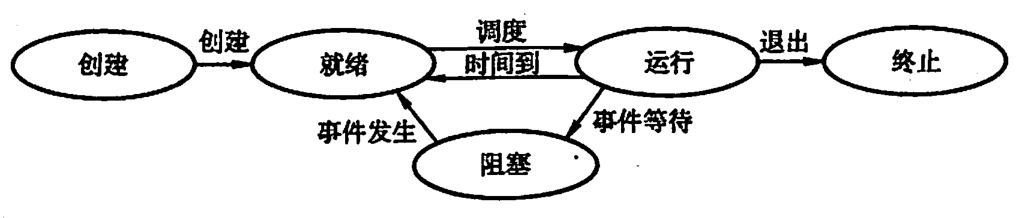
\includegraphics[width=0.7\textwidth]{./images/process_state_transition.png}
  \caption{5种进程状态的转换}
  \label{process_state_transition}
\end{figure}

注意:进程从运行态转换到阻塞态是主动的行为,从阻塞态转换到就绪态是被动的行为。

\subsubsection{进程的组成}

进程实体=程序段+相关的数据段+PCB。本节主要介绍PCB。

PCB包括如下4部分内容:
\begin{itemize}
  \item 进程描述信息。
  \item 进程控制和管理信息。
  \item 资源分配清单。
  \item 处理机相关信息。
\end{itemize}

\subsubsection{进程控制}

本节主要介绍进程的创建、中止、阻塞和唤醒原语的过程。似乎不太重要,暂略。

\subsubsection{进程的通信}

\begin{itemize}
  \item 共享存储
  \begin{itemize}
    \item 分类
    \begin{itemize}
        \item 基于共享数据结构的通信方式
        \item 基于共享存储区的通信方式
    \end{itemize}
    \item 特点
    \begin{itemize}
        \item 适合大量的数据快速交换
        \item 程序员负担重
    \end{itemize}
  \end{itemize}
  \item 消息传递
  \begin{itemize}
    \item 分类:
    \begin{itemize}
        \item 直接通信方式
        \item 间接通信方式:通过信箱(mailbox)通信
        \begin{itemize}
            \item 公有信箱
            \item 私有信箱
            \item 共享信箱
        \end{itemize}
    \end{itemize}
    \item 特点:
    \begin{itemize}
        \item 操作系统隐藏通信细节
        \item 通信程序简单
        \item 可以跨网络传输
        \item 灵活
    \end{itemize}
  \end{itemize}
  \item 管道:通过一个固定大小的共享文件实现通信。UNIX首创。
\end{itemize}

\subsubsection{线程和多线程模型}

传统进程的两个基本属性
\begin{itemize}
    \item 是拥有资源的独立单位
    \item 是调度和分派的基本单位
\end{itemize}

线程的特点:
\begin{itemize}
    \item 是能独立运行的基本单位,且切换代价远小于进程。
    \item 线程不拥有系统资源,而是仅拥有一点必不可少的、能保证独立运行的资源。
    \item 多个线程可以共享一个进程的资源
\end{itemize}

线程的实现:
\begin{itemize}
  \item 用户级线程 ULT:无须内核支持,与内核无关,甚至内核不知道此类线程的存在。调度以进程为单位进行。
  \item 内核级线程 KLT:在内核的支持下运行。调度以线程为单位进行。
\end{itemize}

多线程模型:
\begin{itemize}
  \item 多对一模型,多个用户级线程映射到一个内核级线程。
  \item 一对一模型,每个用户级线程都映射到一个内核级线程。
  \item 多对多模型,将$n$个用户线程映射到$m$个内核级线程上,要求$n\geq m$。
\end{itemize}

\subsection{处理机调度}

\subsubsection{调度的概念}

调度的层次:
\begin{itemize}
  \item 高级调度:又称长程调度、作业调度、接纳调度。
  \begin{itemize}
    \item 调度对象是作业。
    \item 根据某种算法,决定将外存上处于后备队列中的哪几个作业调入内存。
    \item 仅设置在多道批处理系统中。分时系统和实时系统不设置。
    \item 调度频率低,典型时间:几分钟。
    \item 因为调度频率低,调度算法可以设计得很复杂。
  \end{itemize}
  \item 低级调度:又称进程调度或短程调度。
  \begin{itemize}
    \item 调度对象是就绪的进程或内核级线程。
    \item 根据某种算法,决定就绪队列中的哪个进程获得处理机。
    \item 这是最基本的调度方式,在各类OS中都必须设置。
    \item 调度频率高,典型时间:几十毫秒。
    \item 因为调度时间短,调度算法必须足够简单。
  \end{itemize}
  \item 中级调度:又称内存调度。
  \begin{itemize}
    \item 调度对象是就绪进程和阻塞进程。
    \item 其实就是内存对换功能。引入的主要目的是提高内存利用率和系统吞吐量。
  \end{itemize}
\end{itemize}

\subsubsection{调度的性能指标}

\begin{itemize}
  \item CPU利用率:
  \begin{equation*}
    \text{CPU利用率}=\frac{\text{CPU有效工作时间}}{\text{CPU有效工作时间+CPU空闲时间}}
  \end{equation*}
  \item 系统吞吐量:单位时间内完成作业的数量。长作业会降低吞吐量,短作业会提高吞吐量。
  \item 周转时间:从作业被提交给系统开始,到作业完成为止的时间。=等待时间+执行时间。
  \begin{itemize}
    \item 设$T_i$是第$i$个作业的周转时间,$n$为作业总数,则系统的平均周转时间定义为
    \begin{equation*}
        T=\frac{1}{n}\left[\sum_{i=1}^{n}T_i\right]
    \end{equation*}  
    \item 再设$T_{si}$是第$i$个作业的要求服务时间,则系统的平均带权周转时间定义为
    \begin{equation*}
        W=\frac{1}{n}\left[\sum_{i=1}^{n}\frac{T_i}{T_{si}}\right]
    \end{equation*}
  \end{itemize}
  \item 等待时间:进程等待处理机的时间。影响用户满意度。
  \item 响应时间:用户提交请求到系统首次产生相应的时间。
\end{itemize}

\subsubsection{调度的实现}

调度程序的组成:
\begin{itemize}
  \item 排队器
  \item 分派器
  \item 上下文切换器
\end{itemize}

\textbf{不能}进行调度的情况:
\begin{itemize}
  \item 处理中断时。
  \item 进程在OS内核临界区内。
  \item 需要完全屏蔽中断的原子操作。
\end{itemize}

进程调度方式
\begin{itemize}
  \item 非抢占式调度方式:适用于大多数批处理系统,不适用于分时系统和实时系统。
  \item 抢占式调度方式
\end{itemize}

\subsubsection{典型的调度算法}

作业调度算法:
\begin{itemize}
  \item {\bf 先来先服务(FCFS)调度算法}:最简单的调度算法。即可用于作业调度,也可用于进程调度。

  特点:
  \begin{itemize}
      \item 实现简单
      \item 对短作业不公平
  \end{itemize}
  \item {\bf 短作业/短进程优先(SJF/SPF)调度算法}:以作业要求的服务时间长短计算优先级。作业越短,优先级越高。

  特点:
  \begin{itemize}
      \item 实现困难,因为难以估计作业的执行时间。
      \item 有利于短作业。
      \item 对长作业不公平。
      \item 完全没有考虑作业的紧迫程度。
  \end{itemize}
  \item {\bf 优先级调度算法(PSA)}:由外部赋予作业相应的优先级,根据该优先级调度。高优先级作业优先运行。
  \item {\bf 高响应比优先调度算法(HRRN)}:基本思想是动态优先级,作业等待时间越长,优先级越高。
  
  \begin{equation*}
    \text{响应比}R_p=\frac{\text{等待时间+要求服务时间}}{\text{要求服务时间}}=\frac{\text{响应时间}}{\text{要求服务时间}}
  \end{equation*}
  以响应比作为优先级。特点:
  \begin{itemize}
      \item 既照顾了短作业,又考虑了作业到达的先后次序,不会使长作业长期得不到服务。
      \item 每次调度之前要计算响应比,系统开销加大。
  \end{itemize}
\end{itemize}

\begin{problem}
  5个进程A,B,C,D,E分别于0,1,2,3,4时刻到达系统,要求服务时间分别为4,3,5,2,4, 请计算:
  \begin{enumerate}
    \item [(1). ] 采用FCFS时进程执行顺序和平均周转时间;
    \item [(2). ] 采用SPF时进程执行顺序和平均周转时间;
    \item [(3). ] 采用HRRN时进程执行顺序和平均周转时间。
  \end{enumerate}
\end{problem}

\begin{solution}
  \begin{enumerate}
    \item [(1). ]
    进程执行顺序:A$\rightarrow$B$\rightarrow$C$\rightarrow$D$\rightarrow$E\\
    平均周转时间:T = (4+6+10+11+14) / 5 = 9\\
    平均带权周转时间:W=(4/4+6/3+10/5+11/2+14/4) / 5 = 2.8
    \item [(2). ]
    进程执行顺序:A$\rightarrow$D$\rightarrow$B$\rightarrow$E$\rightarrow$C\\
    平均周转时间:T= (4+8+16+3+9) / 5 = 8 \\
    平均带权周转时间:W=(4/4+8/3+16/5+3/2+9/4) / 5 $\approx$ 2.12
    \item [(3). ]
    待补
  \end{enumerate}
\end{solution}

进程调度算法:
\begin{itemize}
  \item {\bf 时间片轮转调度算法(RR)}:让就绪队列上的每个进程每次运行一个时间片长度。

  时间片一般取略大于一次典型的交互所需要的时间,以保证及时响应。
  \begin{itemize}
      \item 时间片太长,则退化为FCFS算法
      \item 时间片太短,调度频繁,浪费资源
  \end{itemize}
  \item {\bf 优先级调度算法}:和作业调度的PSA一致。可以抢占,也可以非抢占。
  \item {\bf 多级反馈队列(MFQ)调度算法}。有如下规则:
  \begin{itemize}
    \item 设置多个就绪队列,为每个队列赋予不同的优先级,第一个队列最高,第二个次之,以此类推。
    \item 优先级越高的队列,执行时间片越小。
    \item 每个队列都采用FCFS算法。一个新进程到来时,将其放到第一个队列的末尾。轮到它执行时,如果不能在一个时间片内完成,则放入第二队列末尾,以此类推。直到放入第n个队列,按照RR算法运行。
    \item 仅当第1队列空闲时,调度程序才调度第2队列中的进程运行;仅当第$1\text{~}(i-1)$队列均空时,才会调度第i队列中的进程运行。
    \item 若第i队列的进程正在执行,此时有新进程进入优先级更高的队列,则立即暂停当前进程并将其放入第i队列的末尾,转而执行新进程。
  \end{itemize}
\end{itemize}

常见进程调度算法的对比:见表\ref{process_handling_algorithms}

\begin{table}
  \centering
  \caption{常见进程调度算法的对比}
  \label{process_handling_algorithms}
  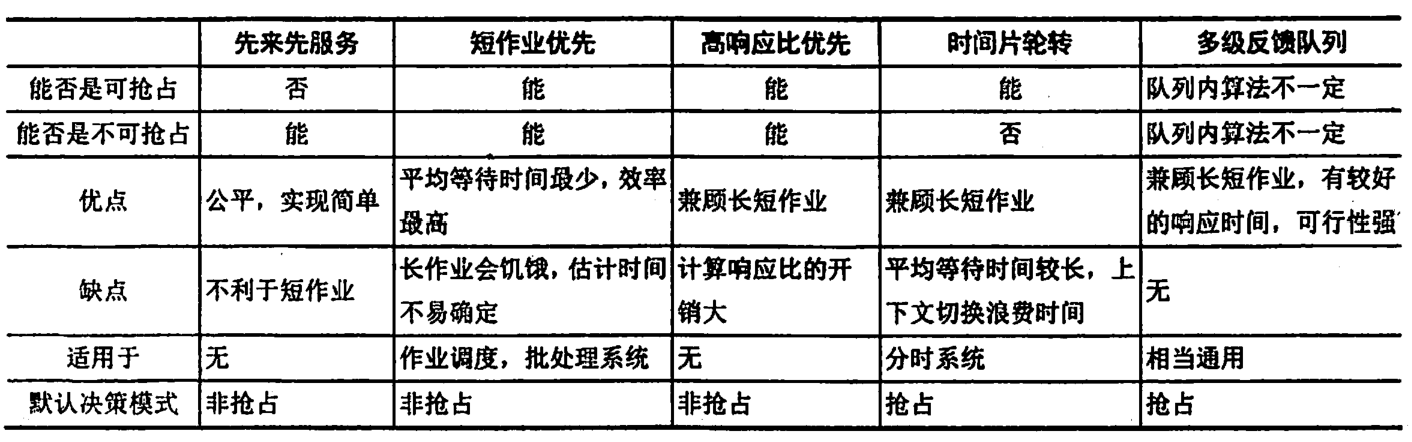
\includegraphics[width=0.9\textwidth]{./images/process_handling_algorithms.png}
\end{table}

\subsubsection{进程切换}

上下文:指某一时刻CPU寄存器和程序计数器的内容。

\begin{itemize}
  \item 上下文切换:从一个进程切换到另一个进程,运行在内核态。
  \item 模式切换:用户态和内核态之间的切换。
\end{itemize}

调度和切换的区别:
\begin{itemize}
  \item 调度是指\textbf{决策}要把资源分配给哪个进程的行为;
  \item 切换是指\textbf{执行}这一切换的行为。
\end{itemize}

\subsection{同步与互斥}

本节的重点是用PV操作解决进程的同步互斥问题。已经多次考察过。

\subsubsection{同步和互斥的基本概念}

\begin{itemize}
  \item {\bf 临界资源}:一次仅允许一个进程使用的资源。访问临界资源的那段代码称为\textbf{临界区}。把临界资源的访问分为4个部分:
  \begin{enumerate}
    \item 进入区:在此处检查能否进入临界区。
    \item 临界区:完成临界资源的访问。
    \item 退出区:将正在访问临界区的标志清除。
    \item 剩余区:代码的其他部分。
  \end{enumerate}
  \item {\bf 同步},又称\textbf{直接}制约关系。指两个或多个进程因需要协调它们的工作次序而等待、传递信息的关系。
  \item {\bf 互斥},又称\textbf{间接}制约关系。进程通过临界资源形成了间接制约关系。原则:
  \begin{enumerate}
    \item \label{kxrj}空闲让进:当无进程处于临界区时,请求进入临界区的进程可立即进入
    \item \label{mzdd}忙则等待:当已有进程进入临界区时,其他试图进入临界区进程须等待
    \item \label{yxdd}有限等待:对要求访问临界资源进程,保证能在有限时间内进入临界区
    \item \label{rqdd}让权等待:当进程不能进入临界区时,应释放处理机
\end{enumerate}

其中\ref{kxrj}和\ref{mzdd}是必须实现的,否则无法实现互斥;
\ref{yxdd}和\ref{rqdd}不实现不会影响互斥,但会严重影响系统的性能。
\end{itemize}

\subsubsection{实现临界区互斥的基本方法}

\begin{itemize}
  \item 软件方法:如Peterson算法
  \item 硬件方法:
  \begin{itemize}
      \item 关中断:CPU仅在中断时才进行进程切换。
      \item 利用Test-and-Set指令
      \item 利用Swap指令
  \end{itemize}
\end{itemize}

\subsubsection{互斥锁 Mutex}

用函数\verb|acquire()|获得锁,用函数\verb|release()|释放锁。二者都是用硬件实现的原子操作。一旦某个进程获得了锁,该锁就不再可用,其他进程试图获得锁时将被阻塞。

主要缺点是有忙等待现象。进程无法获得锁时,必须连续循环调用\verb|acquire()|。

\subsubsection{信号量}

用两个标准的原语\verb|wait(S)|和\verb|signal(S)|访问。也叫P/V操作。

\begin{itemize}
  \item {\bf 整型信号量}
  
  定义一个表示资源数目的信号量S,则
  \begin{lstlisting}
    wait(S) {
      while (S <= 0);
      S -= 1;
    }
    signal(S) {
      S += 1;
    }
  \end{lstlisting}
  还是会有忙等,没有实现让权等待。
  \item {\bf 记录型信号量}
  
  解决了忙等。除了表示资源数目的变量\verb|value|外,还设置一个进程链表L,链接所有等待资源的进程:
  \begin{lstlisting}
    typedef struct {
      int value;
      struct process *L;
    } semaplore;
  \end{lstlisting}
  相应的\verb|wait(S)|和\verb|signal(S)|如下:
  \begin{lstlisting}
    void wait(semaplore S) {
      S.value -= 1;
      if (S.value < 0) {
        add this process to S.L;
        block(S.L);
      }
    }
    void signal(semaplore S) {
      S.value += 1;
      if (S.value <= 0) {
        remove a process P from S.L;
        wakeup(P);
      }
    }
  \end{lstlisting}
  \begin{itemize}
    \item S.value >= 0时,表示资源数量。
    \item S.value < 0时,其绝对值表示被阻塞进程的数量。
  \end{itemize}
\end{itemize}

\subsubsection{管程}

信号量的不足是进程必须手动管理信号量,为OS的统一管理带来了不变。管程解决了这个问题。

管程其实就是一个类:
\begin{lstlisting}
  monitor Demo {
    struct S;   //共享的数据结构
    
    init_code() {
      S = 5;
    }
    take_away() {
      S -= 1;
      //其他操作……
    }
    give_back() {
      S += 1;
      //其他操作……
    }
  }
\end{lstlisting}

\subsubsection{经典同步问题}

四大基本问题
\begin{itemize}
  \item 生产者-消费者问题
  \item 读者-写者问题
  \item 哲学家进餐问题
  \item 吸烟者问题
\end{itemize}

待补!

\subsection{死锁}

\subsubsection{死锁的概念}

死锁的\textbf{定义}:如果一组进程中的每一个进程都在等待仅由该组进程中的其他进程才能引发的事件,那么该组进程是死锁的(Deadlock)。

产生死锁的原因:
\begin{itemize}
  \item 竞争非剥夺性资源(不可抢占资源)
  \item 进程推进顺序不当
\end{itemize}

产生死锁的必要条件,必须同时具备才可能死锁:
\begin{itemize}
  \item 互斥条件:某一段时间内资源只能被一个进程使用,其他进程想用时必须等待。
  \item 请求和保持条件:进程已经得到一部分资源,还需要另一部分资源,但请求的资源已无空闲,因此进程等待,但不释放已经占有的资源。
  \item 不可抢占条件:进程占有资源时,资源不能抢占,只能等进程主动释放。
  \item 循环等待条件:死锁时必然有若干个进程形成了循环等待。
\end{itemize}

死锁的处理策略:
\begin{itemize}
  \item 预防死锁:部分或全部破坏死锁的四个条件。优点是简单,缺点是资源利用率低,效率低。
  \item 避免死锁:进程申请资源时,检查安全性,只有安全才分配资源。优点是效率高一些,缺点是实现困难。
  \item 检测和解除死锁:不做任何限制,定时或资源不足时检查系统中有无死锁,有则解除。优点是效率高。缺点是通过剥夺解除死锁,可能会产生问题。
\end{itemize}

\subsubsection{死锁预防}

预防死锁就是破坏死锁的四个必要条件中的至少一个。互斥条件是不能改变的,因此主要考虑其他三个条件。
\begin{itemize}
  \item 破坏“请求和保持”条件
  \begin{itemize}
    \item 进程创建时,一次申请所有资源。成功则运行,否则阻塞。
    \item 优点:简单,容易实现,安全。
    \item 缺点:资源严重浪费,进程执行大大推迟。
  \end{itemize}
  \item 破坏“不可抢占”条件
  \begin{itemize}
    \item 进程申请资源时,成功则运行,否则释放所有资源后阻塞。
    \item 没有优点。
    \item 缺点:资源严重浪费、代价太大、进程执行进度严重延迟。
  \end{itemize}
  \item 破坏“循环等待条件”
  \begin{itemize}
    \item 为所有资源编号,进程申请资源时必须按序申请资源。
    \item 优点:资源利用率、系统吞吐量显著提高。
    \item 缺点:还是有资源浪费。
  \end{itemize}
\end{itemize}

\subsubsection{死锁避免}

\textbf{系统安全状态}:所谓安全状态,是指系统能按照某种进程推进顺序$(P_1,P_2,\cdots,P_n)$为每个进程$P_i$分配其所需资源,直至满足每个进程对资源的最大需求,使每个进程都顺利完成。此时称$(P_1,P_2,\cdots,P_n)$为安全序列。安全序列是不唯一的。

安全状态下,不会发生死锁;不安全状态下,可能发生死锁。

\vspace*{10pt}

银行家算法:

在系统中设置四个数据结构:
\begin{itemize}
  \item 可用资源向量Available:长度为m的数组,其中每个元素代表一类可利用的资源数目。
  \item 最大需求矩阵Max:n$\times$m的矩阵,表示系统中的n个进程每个对m类资源的最大需求。
  \item 分配矩阵Allocation:n$\times$m的矩阵,表示当前已分配的资源情况。
  \item 需求矩阵Need:n$\times$m的矩阵,表示每个进程还需要的资源数量。
\end{itemize}

上述矩阵存在如下关系:
\begin{equation*}
    \text{Need[i,j]}=\text{Max[i,j]}-\text{Allocation[i,j]}
\end{equation*}

\vspace{10pt}

\textbf{银行家算法的过程}:
设Request$_i$是进程$P_i$的请求向量。当$P_i$发出资源请求后,系统按照如下步骤进行检查:

\begin{enumerate}
  \item [(1). ] 若Request$_i\leq$Need[i,j],转(2);否则出错。
  \item [(2). ] 若Request$_i\leq$Available[j],转(3);否则表示资源不够,$P_i$须等待。
  \item [(3). ] 系统试着把资源分给$P_i$,并进行如下修改:
  \begin{gather*}
    \text{Available[j]}-=\text{Request}_i\text{[j]}\\
    \text{Allocation[i,j]}+=\text{Request}_i\text{[j]}\\
    \text{Need[i,j]}-=\text{Request}_i\text{[j]}
  \end{gather*}
  \item [(4). ] 系统检查当前是否处于安全状态。若是,则正式分配资源;若否,则不分配,令$P_i$等待。
\end{enumerate}

\textbf{安全性算法}:

\begin{enumerate}
  \item [(1). ] 设置两个向量:
  \begin{itemize}
    \item Work向量,长度m,表示系统可以提供给进程的资源数目。算法开始时Work=Available。
    \item Finish向量,长度m,表示系统是否有足够资源分给进程,使之运行完成。开始时Finish[i]=false。
  \end{itemize}
  \item [(2). ] 找到一个能满足下述条件的进程:
  \begin{itemize}
    \item Finish[i]=false;
    \item Need[i,j]$\leq$Work[j];
  \end{itemize}
  若找到,转(3),否则转(4)。
  \item [(3). ] 进程$P_i$获得资源后,可执行至结束,并释放资源。因此执行:
  \begin{gather*}
    \text{Work[j]}+=\text{Allocation[i,j]}\\
    \text{Finish[i]}=\text{True}\\
  \end{gather*}
  然后转(2)。
  \item [(4). ] 若所有进程的Finish[i]都为true,则表示系统处于安全状态,否则为不安全状态。
\end{enumerate}

\subsubsection{死锁的检测和解除}

资源分配图:如图\ref{resource_allocation_graph},圆圈表示进程,方框表示资源。方框里面可以有圆圈,表示该资源有多少个。由资源指向进程的箭头表示该资源\textbf{已经}分配给进程(分配边),由进程指向资源的箭头表示该进程正在请求但\textbf{尚未}得到资源(请求边)。

\begin{figure}
  \centering
  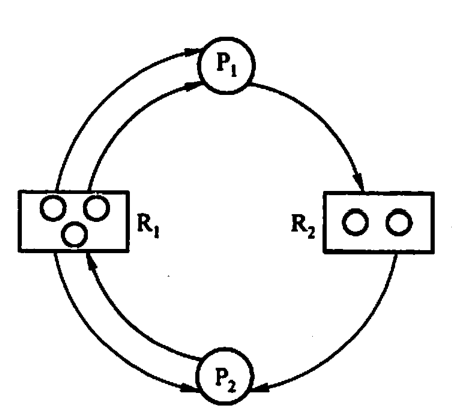
\includegraphics[width=0.5\textwidth]{./images/resource_allocation_graph.png}
  \caption{资源分配图示例}
  \label{resource_allocation_graph}
\end{figure}

资源分配图可以简化:
\begin{enumerate}
  \item 首先找出图中可以得到申请的资源的进程。如图\ref{resource_allocation_graph}的P$_1$申请了一个R$_2$资源,该资源空闲,P$_1$可以得到该资源。如果这种进程没有因得不到资源而阻塞,那么它迟早要运行结束,释放出已经得到的资源。于是将和这种进程相连的所有边删去。
  \item 由于资源的释放,与之相关的进程也可能解除了阻塞状态,考察这些进程,如果它们能够运行结束,就同样删去所有边。
  \item 如此循环,直到不能再删为止。如果此时没有边剩下,就说这个图是可以完全简化的。
  \item 死锁等价于资源分配图不可完全简化。这叫做死锁定理。
\end{enumerate}

一些解除死锁的方法:
\begin{itemize}
  \item {\bf 资源剥夺法},挂起占有资源的进程,将其资源剥夺,分配给其他进程。注意不能挂起太久。
  \item {\bf 撤销进程法},直接杀掉占有资源的进程,将资源分给其他进程。杀的顺序可以是进程优先级或代价的高低。
  \item {\bf 进程回退法},OS保存进程的历史信息,要求一些进程主动回退,释放出一些资源。
\end{itemize}

\subsection{本章疑难点}

饥饿进程:和死锁不一样,指的是由于OS的分配策略不完美而引发某个进程一直等待的情况。例如在短进程优先调度中,短进程源源不断地进来,长进程一直排队而无法运行。如果饥饿进程被耽误的时间太长,导致即使完成也无济于事(有时效)时,称这个进程被“饿死”。

\section{内存管理}

\subsection{内存管理概念}

\subsubsection{内存管理的基本原理和要求}

内存管理的主要任务:
\begin{itemize}
  \item 内存空间的分配和回收
  \item 地址转换
  \item 内存空间扩充
  \item 内存共享
  \item 存储保护
\end{itemize}

程序的链接:
\begin{itemize}
  \item 静态链接:编程时,链接所有模块
  \item 装入时动态链接:装入时,链接所有模块
  \item 运行时动态链接:运行时,根据需要链接模块
\end{itemize}

程序的装入:
\begin{itemize}
  \item \textbf{绝对装入方式}:编译时直接确定装入的内存位置,装入后无需再修改程序和数据的地址。用于单道程序环境。
  \item \textbf{可重定位装入方式}:用于多道程序环境。装入时对逻辑地址修改得到物理地址,又称\textbf{静态(地址)重定位}。程序在内存中不能移动。
  \item \textbf{动态运行时的装入方式}:相对于上面的装入时进行重定位,本方式在程序执行时才进行重定位。又称\textbf{动态(地址)重定位}。需要重定位寄存器的支持。
\end{itemize}

进程的内存映像包括:
\begin{itemize}
  \item 代码段:只读
  \item 数据段:包括全局变量和静态变量
  \item PCB
  \item 堆
  \item 栈
\end{itemize}

\begin{figure}
  \centering
  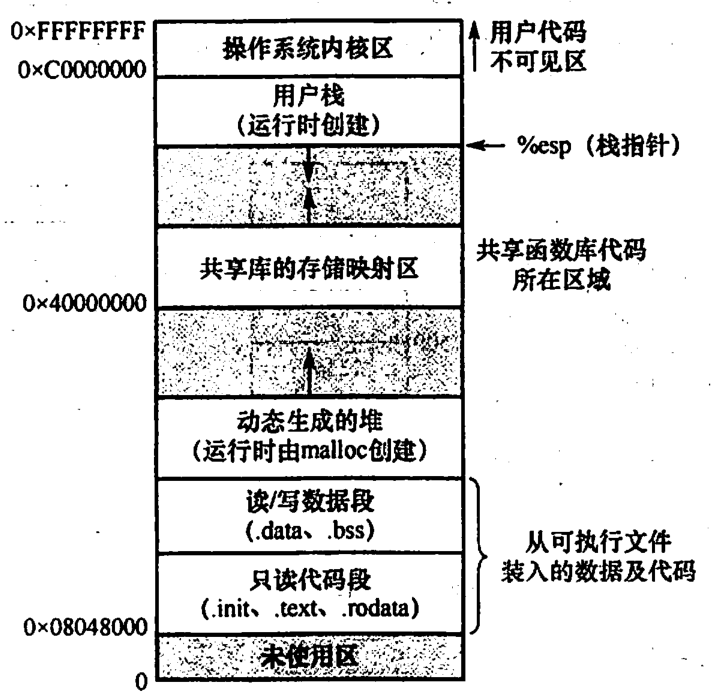
\includegraphics[width=0.6\textwidth]{./images/process_in_memory.png}
  \caption{内存中的一个进程}
\end{figure}

\subsubsection{覆盖与交换}

本节已从新大纲中删除。了解即可。参见王道OS2024版P177(书的P164)。

\subsubsection{连续分配管理方式}

最早出现的一种存储器分配方式,该方式为用户分配一个连续的内存空间。

内存的零头:
\begin{itemize}
  \item 内零头:分配给进程,而进程未用到的内存部分;
  \item 外零头:未分配给进程,但因为太小而无进程能用;
\end{itemize}

\begin{itemize}
  \item {\bf 单一连续分配}
  \begin{itemize}
    \item 主要用于单用户OS。在一段时间内,只有一个进程在内存。
    \item 基本思想:内存分为两个区域:一个供操作系统使用,一个供用户使用。
    \item 三种典型的布局方式:
    \begin{itemize}
      \item 用户空间在低地址,系统空间在高地址。
      \item 和上面反过来。
      \item 系统空间在两边,把用户空间夹起来。
    \end{itemize}
    \item 实现:设置基址寄存器、限界寄存器,要求逻辑地址映射为物理地址后,物理地址必须在两者之间。
    \item 特点:简单,适用于单任务OS
  \end{itemize}
  \item {\bf 固定分区分配}
  \begin{itemize}
    \item 用于多道程序系统。把内存划分为固定的几个部分,维护一个分区使用表。示例见表\ref{area_table_example}。
    \item 特点:
    \begin{itemize}
      \item 最早的支持多道程序的内存管理方式。
      \item 简单,现在仍在嵌入式系统中应用。
      \item 内零头严重。
    \end{itemize}
  \end{itemize}
  \item {\bf 动态分区分配}
  \begin{itemize}
    \item 基本思想:程序运行时划分大小合适的分区,程序结束后收回分区
    \item 配套数据结构:
    \begin{itemize}
      \item 空闲分区表:和固定分区一样
      \item 空闲分区链:在分区头部放入必要的说明信息和前向指针,分区尾部放入后向指针。
    \end{itemize}
    \item 动态分区分配算法:分为分配算法和回收算法两部分。分配算法又分基于顺序搜索的算法和基于索引搜索的算法两部分。
    \item 回收算法比较简单,在回收内存之后要做:
    \begin{itemize}
      \item 上下两个相邻区都是空闲区时,合并三个区
      \item 上空闲下不空闲时,合并上面的区
      \item 下空闲上不空闲时,合并下面的区
      \item 上下都不空闲时,不合并。
    \end{itemize}
    \item 基于顺序搜索的分配算法:用于小型系统
    \begin{itemize}
      \item 首次适应算法
      \begin{itemize}
        \item 低地址端被快速分配,碎片迅速出现
        \item 高地址端可能出现大块空闲区
      \end{itemize}
      \item 循环首次适应算法
      \begin{itemize}
        \item 需要设置一个查找指针
        \item 本质是CLOCK算法
        \item 碎片分布均匀
      \end{itemize}
      \item 最佳适应算法
      \begin{itemize}
        \item 需要将空闲区按照从小到大的顺序形成一个链,第一次找到的能放下的分区一定是最佳的。
        \item 碎片会迅速出现,实际上是很差劲的算法。
      \end{itemize}
      \item 最坏适应算法
      \begin{itemize}
        \item 仍然形成空闲分区链,但顺序是从大到小,每次只检查第一个(最大的)分区能否满足要求。
        \item 碎片出现最慢,但优先使用大内存块,导致很快就没有可用的大内存块了,同样是很差劲的算法。
      \end{itemize}
    \end{itemize}
    \item 基于索引搜索的分配算法:用于大中型系统
    \begin{itemize}
      \item 快速适应算法
      \item 伙伴系统
      \item 哈希算法
    \end{itemize}
  \end{itemize}
  \item {\bf 可重定位分区分配}
  \begin{itemize}
    \item 在动态分区分配的基础上引入”紧凑“机制,消除外零头。使用动态地址重定位。
  \end{itemize}
\end{itemize}

\begin{table}[!ht]
  \centering
  \caption{分区说明表示例}
  \label{area_table_example}
  \begin{tabular}{|c|c|c|c|}
  \hline
    \textbf{区号} & \textbf{分区长度(KB)} & \textbf{起始地址} & \textbf{状态} \\ \hline
    1 & 12 & 20 & 已分配 \\ \hline
    2 & 32 & 32 & 已分配 \\ \hline
    3 & 64 & 64 & 未分配 \\ \hline
    4 & 128 & 128 & 已分配 \\ \hline
  \end{tabular}
\end{table}

\subsubsection{基本分页存储管理}

与连续分配相对,有离散分配方式,分为以下三类:
\begin{itemize}
  \item 分页存储管理方式
  \item 分段存储管理方式
  \item 段页式存储管理方式
\end{itemize}

页面不宜太大,也不宜太小,太大内存利用率低,太小又浪费内存。
一般为2的整数次方,1KB-8KB。

快表:待补

多级页表:待补

\subsubsection{基本分段存储管理}

按照用户进程中的自然段划分逻辑空间。段内要求连续,段间不要求连续。逻辑地址=段号+段内偏移量

页式系统中内存管理对用户透明,段式系统中则要求编译器管理段号和偏移量。

段表:每个进程都有一张段表,其中的每个项对应进程的一段。包含3个域:段号、段长、本段在内存的起始地址。

\subsubsection{段页式管理}

段页式系统中,逻辑地址分为三部分:段号、页号和页内偏移量。

系统为每个进程建立一张段表,每个分段有一张页表。

地址变换时,先通过段表查找页表始址,然后通过页表查找到页帧号,最后形成物理地址,需要三次访存。

\subsection{虚拟内存管理}

\subsubsection{虚拟内存的基本概念}

存储管理的两个基本问题:
\begin{itemize}
  \item 有的作业很大,不能完整装入内存。
  \item 作业很多,不能全部放入内存,但它们又要求同时运行。
\end{itemize}

程序运行的局部性原理:
\begin{itemize}
  \item 时间局部性:刚执行过的指令在不久后很可能再次被执行,或程序刚访问过的数据很可能再次被访问。典型原因是程序中的循环。
  \item 空间局部性:程序刚访问过某存储单元,则附近的存储单元也很可能被访问。典型原因是程序的顺序执行。
\end{itemize}

\textbf{定义}:虚拟存储器是指具有请求调入功能和置换功能,能从逻辑上对内存容量加以扩充的一种存储器系统。其逻辑容量由内存容量和外存容量之和决定,运行速度接近内存速度,而每位的成本由接近外存。

特征:
\begin{itemize}
  \item 多次性。程序无须一次性全部装入内存,而是可以分多次装入。
  \item 对换性。程序和数据无须常驻内存,在必要时可以换入换出。
  \item 虚拟性。能从逻辑上扩展内存容量,使用户看到的容量远大于实际容量。
\end{itemize}

实现方法:
\begin{itemize}
  \item 请求分页系统
  \item 请求分段系统
  \item 请求段页系统
\end{itemize}

需要的硬件支持:
\begin{itemize}
  \item 一定容量的内存和外存。
  \item 页表/段表机制,作为主要的数据结构。
  \item 中断机构。
  \item 地址变换机构。
\end{itemize}

\subsubsection{请求分页管理方式}

为了应对页不在内存的情况,针对基本分页系统的页表结构进行扩充,形成如图\ref{page_request_system}的结构。

\begin{figure}[h]
  \centering
  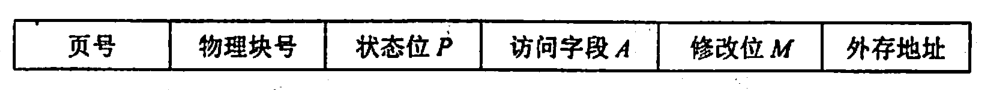
\includegraphics[width=0.9\textwidth]{./images/page_request_system.png}
  \caption{请求分页系统中的页表项}
  \label{page_request_system}
\end{figure}

\begin{itemize}
  \item 状态位P:标示当前页面是否在主存。
  \item 访问字段A:记录一段时间内被访问的次数,供置换算法参考。
  \item 修改位M,标示该页面在被调入内存后是否被修改过。
  \item 外存地址:指出该页面在外存的地址。
\end{itemize}

请求分页系统的地址变换过程:图\ref{page_request_address_translation}

\begin{figure}
  \centering
  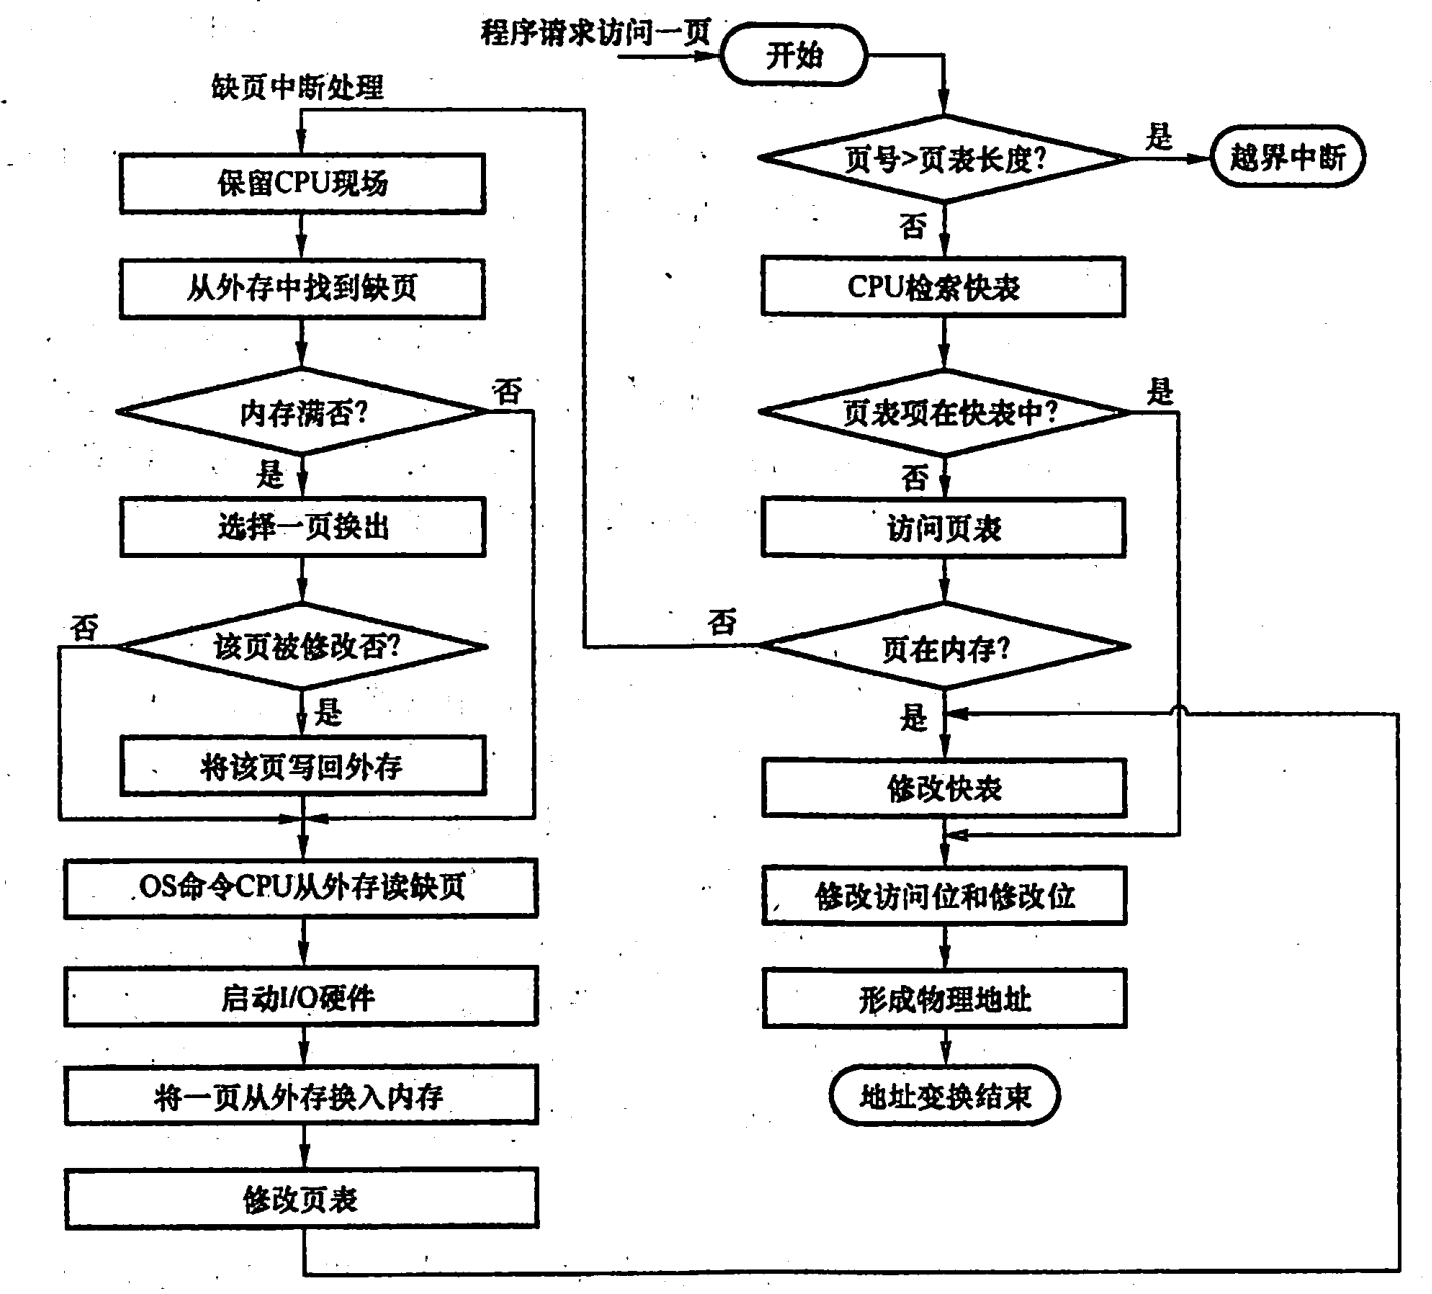
\includegraphics[width=0.7\textwidth]{./images/page_request_address_translation.png}
  \caption{请求分页系统中的地址变换过程}
  \label{page_request_address_translation}
\end{figure}

\subsubsection{页框分配}

给一个进程分配的物理页框的集合,叫做这个进程的\textbf{驻留集}。

内存分配策略:所谓固定分配,是指每个进程分配一定数目的物理块,其大小在进程运行过程中不再改变。所谓全局置换,是指如果进程缺页,则从全局的空闲块中分配,不仅限于该进程自身分配的块。
\begin{itemize}
  \item {\bf 固定分配局部置换}
  \item {\bf 可变分配全局置换}
  \item {\bf 可变分配局部置换}
  不是很明白,待补
\end{itemize}

物理块调入算法:仅限于固定分配策略。
\begin{itemize}
  \item 平均分配算法
  \item 按比例分配算法
  \item 优先级分配算法
  细节待补
\end{itemize}

调入页面的时机:
\begin{itemize}
  \item 预调页策略
  \item 请求调页策略
  细节待补
\end{itemize}

从何处调入页面:
\begin{itemize}
  \item 细节待补
\end{itemize}

如何调入页面

\subsubsection{页面置换算法}

选择换页时调出哪一页的算法称为页面置换算法。

\begin{enumerate}
  \item {\bf 最佳(OPT)置换算法}:理论上最优的算法
  \item {\bf 先进先出(FIFO)页面置换算法}:每次都淘汰在内存中驻留时间最久的页面。没有考虑局部性,因此效果不佳。还会出现分配的物理块数增多但页故障数不减反增的\textbf{Belady异常}现象。OPT和LRU则不会出现。该算法基于队列实现。
  \item {\bf 最近最久未使用(LRU)置换算法}:效果良好。该算法基于堆栈实现,需要额外的堆栈和寄存器硬件。可以证明,基于堆栈实现的算法不会出现Belady异常。
  \item {\bf 时钟(CLOCK)置换算法}
  
  是低配的LRU,目的是用更少的硬件资源实现和LRU相近的性能。叫做CLOCK的原因是这种算法的工作方式就像钟表一样循环往复。
  \begin{itemize}
    \item {\bf 简单的CLOCK置换算法}
    
    为每页设置一个访问位A。将所有页视作一个循环队列,并设置一个替换指针。某一页被替换时,将指针指向该页的下一页。如果需要换页,则检查当前指向的页的访问位。如果是0,则换出;如果是1,则置为0(再给一次机会)。如此循环扫描,直到找到0为止。
    \item {\bf 改进的CLOCK置换算法}
    
    这种改进将页面是否被更改过也纳入了考虑。更改的页面需要真正写入磁盘,未更改的页可以简单丢弃,故更改的页换页代价更高。为每页再增加一个修改位M。扫描过程如下:
    \begin{enumerate}
      \item 第一趟扫描,寻找A=0且M=0的页。这种页替换代价最小,一旦找到就停止扫描,将该页换出。若未找到,则开始第二趟。这一趟\textbf{不修改A}。
      \item 第二趟扫描,寻找A=0且M=1的页。一旦找到就停止扫描,将该页换出。若未找到,则开始第三趟。这一趟\textbf{将所有=1的A置为0}。
      \item 第三趟扫描,将所有A置为0,然后按第一趟的逻辑扫描,若还不满足,则按第二趟的逻辑扫描。此时一定可以找到换出的页。
    \end{enumerate}
  \end{itemize}
\end{enumerate}

\subsubsection{抖动和工作集}

\textbf{抖动}:刚刚换入的页马上就要换出,刚刚换出的页马上就要换入,如此持续换页。

抖动发生的\textbf{根本原因是}:系统中的进程太多,分给每个进程的物理块太少。

\textbf{工作集}是指在某段时间内,进程要访问的页面集合。工作集的大小$W$可由工作集窗口$\Delta$和时间$t$确定。对于局部性好的程序,工作集的大小一般远远小于工作集窗口的大小。

为了避免发生抖动,一般要为进程分配大于其工作集的物理块数。

\section{文件管理}

\subsection{文件系统基础}

\subsubsection{文件的基本概念}

文件的结构:
\begin{itemize}
  \item 数据项,是最低级的数据组织形式。可分为:
  \begin{itemize}
    \item 基本数据项,是数据中的最小逻辑单位。
    \item 组合数据项,由多个基本数据项组成。
  \end{itemize}
  \item 记录,是一组相关的数据项的集合,用于描述一个对象在某方面的属性。
  \item 文件,是指由创建者所定义的、具有文件名的一组相关元素的集合。可分为有结构文件和无结构文件。有结构文件由若干个相似的记录组成,无结构文件则是一个字符流,如二进制文件或字符文件。
\end{itemize}

\subsubsection{文件控制块和索引结点}

文件的属性:
\begin{itemize}
  \item 文件名
  \item 文件类型
  \item 创建者
  \item 所有者
  \item 位置
  \item 大小
  \item 保护访问控制信息
  \item 创建时间、最后修改时间和最后存取时间。
\end{itemize}

OS通过文件控制块(FCB)来维护文件的属性。

FCB包含如下信息:
\begin{itemize}
  \item 基本信息,如文件名、文件物理位置、文件的逻辑结构、文件的物理结构。
  \item 存取控制信息,如文件所有者的存取权限、核准用户的存取权限及一般用户的存取权限。
  \item 使用信息,如文件建立时间、上次修改时间等。
\end{itemize}

索引结点:查找文件目录时,要频繁访问硬盘,但查找文件实际上只需要文件名。因此可以将文件名单独抽取出来,搭配指向文件的指针,可以加速查找。这种文件名+指针的数据结构称为索引结点,也叫i节点(inode)。

索引结点可以放在磁盘中,也可以预读入内存。

\subsubsection{文件的操作}

文件的基本操作
\begin{itemize}
  \item 创建。有两个步骤:分配外存空间、为其创建目录项。
  \item 写文件。通过系统调用完成。系统需要查找目录以找到文件,还要维护写指针。
  \item 读文件。同上。维护读指针。一般一个进程不可能同时读和写同一个文件,因此读写指针可以合并起来。
  \item 重新定位文件。查找指定的文件,并将读写指针复位。
  \item 删除文件。找到文件对应的目录项,释放外存空间,并删除这一目录项。
  \item 截断文件。也就是清空文件,但不删除文件。
\end{itemize}

\subsubsection{文件保护}

文件保护通过口令保护、加密保护和访问控制等方式实现。

\subsubsection{文件的逻辑结构}

\begin{itemize}
  \item 逻辑结构是从用户角度出发看到的文件组织形式。
  \item 物理结构(存储结构)是从实际角度出发看到的文件组织形式。
\end{itemize}

按照是否有结构,可将逻辑结构分为:
\begin{itemize}
  \item 有结构文件(记录式文件)
  \begin{itemize}
    \item 定长记录:检索容易
    \item 变长记录:灵活,但只能顺序查找。为此可以设置索引表,索引表本身是定长记录的。
  \end{itemize}
  \item 无结构文件(流式文件)
\end{itemize}

按照文件的组织方式,将有结构文件分为以下四类:
\begin{itemize}
  \item 顺序文件
  
  顺序文件的记录是定长记录或可变长记录。
  \begin{itemize}
    \item 最佳应用场合:对文件中的记录进行批量存取时。
    \item 若共有$N$个记录,则查找一个记录平均需要查$N/2$次。即查找性能不好。
    \item 此外添加或删除一个记录也很困难。可以引入一个事务文件,保存一段时间内的新增和删除记录,每隔一段时间进行实际写入。
  \end{itemize}

  为了访问顺序文件中的记录,必须首先找到记录的地址。有两种方法:
  \begin{itemize}
    \item 隐式寻址:就是从头找起,无论记录是定长的还是不定长的。
    \item 显式寻址:仅能用于寻址定长记录文件,直接将基址加上偏移量得到,由于定长,偏移量很容易得到。
  \end{itemize}
  \item 索引文件
  \begin{itemize}
    \item 主要用于解决变长记录文件的快速查找问题。
    \item 方法:建立一张索引表,其中保存有每个记录的“指针”,是定长的,这样就可以按照关键字查找索引表,然后再跳转到实际记录。
    \item 也可以建立多个索引表,从而支持按照多个属性进行索引。
    \item 缺点是索引表须占用额外存储空间,尤其当记录数量很大时。
  \end{itemize}
  \item 索引顺序文件
  \begin{itemize}
    \item 顺序文件和索引文件的一种折中。
    \item 将记录分组,为每组记录在索引表中建立一个项。
    \item 分组方式:按关键字分组,或直接按记录号分组。
    \item 查找过程:首先查索引表,找到待查项所在的组,通过指针跳转,再在组中顺序查找。
    \item 可以引入多级索引。
  \end{itemize}
  \item 直接文件或散列文件
  \begin{itemize}
    \item 存取速度很快,但是可能会有冲突。
  \end{itemize}
\end{itemize}

正规OS:顺序文件+暴露读写指针

\subsubsection{文件的物理结构}

文件的物理结构实际上就是研究文件数据在物理设备上是如何分布和组织的。这个问题有两个方面:
\begin{itemize}
  \item 文件的分配方式,讲的是非空闲盘块的管理。
  \item 文件的存储空间管理,讲的是空闲盘块的管理。
\end{itemize}

\section{输入输出(I/O)管理}

\end{document}